\documentclass{thesisKGI}

  %------------------- TITULNÍ STRANA ------------------- 

  \title{SYNCHRONIZACE A REPLIKACE GEODAT V PROSTŘEDÍ ESRI PLATFORMY}
  \author{Markéta SOLANSKÁ}
  \thesistype{Magisterská práce}
  \advisor{RNDr. Vilém Pechanec, Ph.D.}

  \bibliographystyle{csplainnat} %styl citací


  \begin{document}
    \sloppy       %lepší hlídání přetékajících řádků
    \maketitle    %vložení titulní strany

    %----------------------------------------------------------------------------------- ČESTNÉ PROHLÁŠENÍ

    %vložení prohlášení, třída se sama postará o tvorbu nové stránky a vloží pod text řádek s datumem a jménem
    \begin{declaration}
      \textbf{Čestné prohlášení}

      Prohlašuji, že jsem magisterskou práci magisterského studia oboru Geoinformatika vypracovala samostatně pod vedením RNDr. Viléma Pechance, Ph.D.

      Všechny použité materiály a zdroje jsou citovány s ohledem na vědeckou etiku, autorská práva a zákony na ochranu duševního vlastnictví.

      Všechna poskytnutá i vytvořená digitální data nebudu bez souhlasu školy poskytovat.
    \end{declaration}

    %----------------------------------------------------------------------------------- PODĚKOVÁNÍ
    
    %poděkování, pokud nějaké chcete uvést, jinak lze tuto sekci smazat
    \begin{dedication}
      Děkuji vedoucímu práce RNDr. Vilému Pechancovi, Ph.D. za podněty a připomínky při vypracování práce.

      Dále děkuji konzultantu XXXXXXXXXX za …..
      Za poskytnutá data děkuji Českému statistickému úřadu, XXXXXXXXXXXXX.
      Za poskytnuté rady a materiály děkuji firmě XXXXXXXXXX.
      \vspace{4em}
    \end{dedication}

    %----------------------------------------------------------------------------------- NASTAVENÍ POČÍTADLA, ZKRATKY
    
    \setcounter{page}{5}          %nastavení počítadla stránek na správnou hodnotu
    \makeTableOfContent{3}        %vložení obsahu, standardně se používají 3 úrovně
    \makeGlossary                 %formát v nemž se vkládají zkratky, vlouží se pouze ty, které budou použity v textu. v textu vkládáme zkratku pomocí příkazu \gls{DTM}
    %vložení seznamu zkratek, smazat, pokud není třeba
      \newglossaryentry{CAD}{name=CAD, description={Computer Aided Design}}
      \newglossaryentry{GIT}{name=GIT, description={geoinformační technologie}}
      \newglossaryentry{SQL}{name=SQL, description={Structured Query Language}}

    %----------------------------------------------------------------------------------- ÚVOD
    %protože je Úvod nečíslovaný je potřeba ho manuálně vložit do obsahu
    \addcontentsline{toc}{section}{Úvod}
    \section*{Úvod}

      Úvod je v rozsahu jedné strany. Je důležitou součástí práce. Uvádí
      do problematiky řešené v bakalářské / magisterské práci. Student v
      něm vyjadřuje potřebu řešení zadaného tématu, případně návaznost na
      jeho předcházející práce. Doporučuje se, aby byl do své konečné
      podoby dopsán až jako poslední, tj. až po napsání celého textu.

      Dnešní trend je stále více dat ukládat a ponechávat pouze v
      digitální podobě. Mnoho dokumentů už se vůbec netiskne do papírové
      podoby. Tento trend dnes podporují i elektronické podpisy, díky
      kterým je tištěná verze naprosto zbytečná. S přibývajícím počtem
      dat je však třeba řešit komplikace, které počítačová data přináší.
      Počítačoví experti řeší například kam ukládat tak velké množství
      dat, jak data aktualizovat, jak zabránit poškození dat ať už
      způsobených lidským faktorem či poškozením hardwaru. V připadě, že
      se poškodí disk, můžeme často během okamžiku přijít o všechna
      data, někdy však pro ztrátu dat stačí stikntou pouhé jedno
      tlačítko na klávesnici. Určitě už se vám nejednou stalo, že jste
      se nemohli přihlásit do svého účtu na internetu z důvodu přetížení
      serveru. Jak zabránit těmto komplikacím, které mohou poškodit či
      zcela zničit celou dosavadní práci nebo zrychlit celý proces práce
      s tady? Řešením velkého počtu výše uvedených problémů je replikace
      dat. Jedná se pokročilou funkci, kterou nabízí dnešní databázové
      servery, zajišťující robustnost databáze a vysokou dostupnost dat
      tím, že data zkopíruje na více serverů.
      
      Replikaci lze využít ve všech odvětvích, které pracují s daty.
      Výjimkou tedy není ani geoiformatika, která pracuje s velkým
      počtem dat, které navíc nesou informaci o geografické poloze. Z
      mého pohledu data středně velkého nebo velkého projektu je
      nejvhodnější ukládata do databáze. Nabízí nám to sofistikované
      uložení dat, snadné propojení jednotlivých vrstev, snadnou
      přenostitelnost dat a další. Replikace se dá využít pro kopii 
      dat a následnou aktualizaci změn. Výhodou databáze je, že se při
      změně jednoho prvku, aktualizuje v databázi pouze jeden řádek a
      nekopíruje se znovu celá databáze, což je jednoznačná výhoda
      oproti binárnímu uložení dat napřiklad ve formátu shapefile.
      
      Replikaci ocení určitě i uživatelé, které pracují na jednom
      projektu. Z hlediska rychlosti práce s databází je výhodnější mít
      databázi přimo na počítači, na kterém pracují, než data in-real
      time stahovat ze serveru. Po dokončení editace se data replikují
      prostřednictvím počítačové sítě nebo internetu. Dobrým příkladem
      využitelnosti replikace je také nový trend využívání offline
      mobilních aplikací v mobilních telefonech. Databáze se vždy
      replikuje do mobilního telefonu, vždy když se klient připojít na
      internetovou síť, aplikace kontroluje zda není na serveru novější
      verze databáze a pokud je, zkopíruje pouze změny, které proběhly
      od posledního stahování. (Jako příklad z geoinformatického
      prostředí bych uvedla diplomovou práci Dalibora Janáka, který řeší
      replikaci databáze lezeckých cest do mobilní aplikace.) Databázové
      systémy nabízí širokou škálu nastavitelnosti, která umožňuje
      přizpůsobit replikaci danému řešení. 

    
    %----------------------------------------------------------------------------------- CÍLE PRÁCE
    %každou kapitolu je třeba začít na nové stránce
    \newpage
    \section{CÍLE PRÁCE}

      Cílem diplomové práce je provést rešerši a na jejím základě
      prakticky otestovat proces synchronizace a replikace geodat, které
      se dnes objevují napříč platformou Esri. V teoretické části práce
      bude detailně analyzován proces synchronizace a replikace ve všech
      možných variantách (jednosměrná, dvousměrná, synchronní,
      asynchronní, ...) a popsány prostředky, které se na platformě Esri k
      těmto procesům využívají. Rozbor zahrne celé portfólio produktů od
      desktop řešení, přes možnosti ArcGIS serveru až po cloudový ArcGIS
      online. Budou popsány možnosti, požadavky a předpoklady pro úspěšnou
      realizaci.

      V praktické části, nad existujícími katedrálními daty, dojde k
      praktickému testování těchto procesů na předem připraveném
      testovacím prostředí. Postupnými opakovanými procesy budou sledovány
      dílčí parametry procesu (rychlost procesu, úplnost, chybovost,
      podporované formáty). Vyjde se z primárně podporovaného databázového
      stroje SQL Server, který bude konfrontován s možnosti dalšího
      podporovaného systému PostgeSQL.

      Můj jeden odstaveček - něco jako - jak vidím vlastní přínos do tématu. 


    %----------------------------------------------------------------------------------- POUŽITÉ METODY A POSTUPY PRÁCE
    \newpage
    \section{POUŽITÉ METODY A POSTUPY PRÁCE}
       \subsection{Obrázky}

    %ukázka zápisu kódu pro obrázek
    %parametr H říká že to bude přímo na tom místě kde je v textu...více http://en.wikibooks.org/wiki/LaTeX/Floats,_Figures_and_Captions
    \begin{figure}[H]
      \centering
      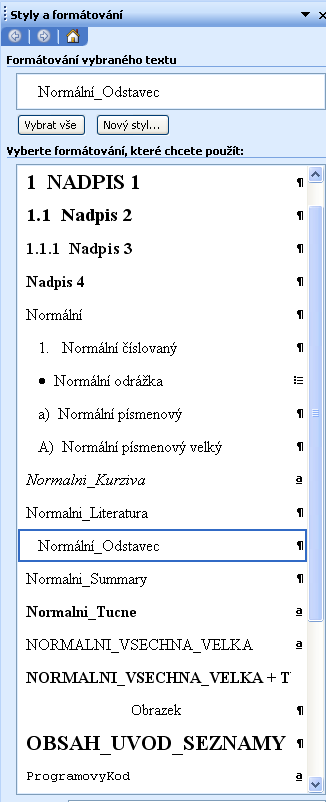
\includegraphics[width=0.2\textwidth]{./obrazky/obrazek_1.png}
      \caption {Styly (převzato z: \cite{Celikyilmaz2009})}
      \label{fig:44}
    \end{figure}

    %ukázka odkazu na zkratky a obrázek
    \Gls{GIT} \Gls{CAD} bla bla bla \odkazObrazek{fig:44}. Pokud chceme uvést překlad z angličtiny můžeme to udělat takto \transl{english words}.

    %dají se dělat i složené obrázky
    \begin{figure}
        \centering
        \begin{subfigure}[b]{0.45\textwidth}
          \centering
          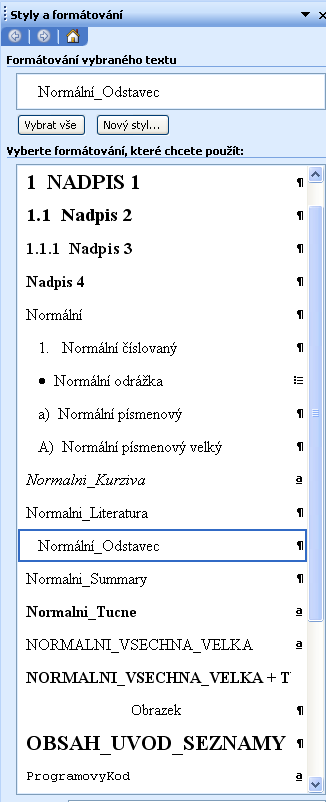
\includegraphics[width=\textwidth]{./obrazky/obrazek_1.png}
          \caption{Cena za metr čtvereční bytů v Londýně (převzato z:\cite{Fotheringham2002})}
          \label{fig2.1}
        \end{subfigure}%
        \quad %add desired spacing between images, e. g. ~, \quad, \qquad etc.
          %(or a blank line to force the subfigure onto a new line)
        \begin{subfigure}[b]{0.45\textwidth}
          \centering
          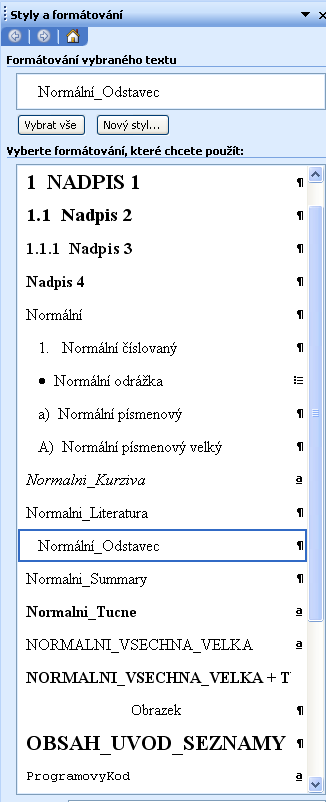
\includegraphics[width=\textwidth]{./obrazky/obrazek_1.png}
          \caption{Obsah zinku v půdě (převzato z:\cite{Hengl2009})}
          \label{fig2.2}
        \end{subfigure}
        \caption{Povrch socioekonomického (a) a fyzickogeografického (b) ukazatele}
        \label{fig2}
    \end{figure}

    \begin{table}[h]
    \caption {Ukázková tabulka}
    \label{tab1}
    \centering
      \begin{tabular}{ |l|l|l| }
        \hline
        \multicolumn{3}{ |c| }{Team sheet} \\
        \hline
        Goalkeeper & GK & Paul Robinson \\ \hline
        \multirow{4}{*}{Defenders} & LB & Lucus Radebe \\
        & DC & Michael Duberry \\
        & DC & Dominic Matteo \\
        & RB & Didier Domi \\ \hline
        \multirow{3}{*}{Midfielders} & MC & David Batty \\
        & MC & Eirik Bakke \\
        & MC & Jody Morris \\ \hline
        Forward & FW & Jamie McMaster \\ \hline
        \multirow{2}{*}{Strikers} & ST & Alan Smith \\
        & ST & Mark Viduka \\
        \hline
      \end{tabular}
    \end{table}

    Odkaz na tabulku pak vytvoříme takto: \odkazTabulka{tab1}.

    \begin{equation}
    \label{eq1}
    c = \sqrt{a^2 + b^2}
    \end{equation}

    Vzorce pak odkazujeme \odkazVzorec{eq1}. 

    Citace se dají dělat buď jako \citep{Talasova2003} nebo \cite{Talasova2003}.



    
    %----------------------------------------------------------------------------------- TEORETICKÁ VÝCHODISKA
    \newpage
    \section{TEORETICKÁ VÝCHODISKA}
    
    %----------------------------------------------------------------------------------- VÝSLEDKY
    \newpage
    \section{VÝSLEDKY}

    %----------------------------------------------------------------------------------- DISKUZE
    \newpage
    \section{DISKUZE}

    %----------------------------------------------------------------------------------- ZÁVĚR
    \newpage
    \section{ZÁVĚR}

    %----------------------------------------------------------------------------------- LITERATURA
    \newpage
    %\makeBibliography{literatura}
    \bibliography{literatura}

    %----------------------------------------------------------------------------------- SUMMARY
    \begin{summary}
      There is summary of all aims, methods and results in this chapter.
      Summary is not only translation of chapter Závěr. There is more
      information from chapters Cíle, Výsledky and Diskuze. Number of
      pages of Summary chapter is two at least. The style is Normalni
      Summary. Language is set to Angličina(Velká Británie) for automatic
      spell check. Do not use language Angličtina(USA). 
    \end{summary}

  \end{document}
